\setcounter{equation}0
\newcommand{\red}[1]{#1}
\newcommand{\add}[1]{#1}
\newcommand{\nnote}[1]{}
\newcommand{\note}[1]{}
\newcommand{\uunit}[1]{[#1]}

\newcommand{\ddlink}[3]{\href{#1}{$\Delta^{#2}\sb{#3}$}}
\spis{Trzecie prawo Keplera i~analiza wymiarowa}
{Grzegorz Łukaszewicz}

\wtyt{Trzecie prawo Keplera\\ i~analiza~wymiarowa}

\waut{Grzegorz ŁUKASZEWICZ*}
\aafil{Wydział Matematyki, Informatyki i~Mechaniki, Uniwersytet Warszawski}


{\it Drogi, którymi ludzie dochodzą do poznania niebios, wydają mi się nie mniej godne podziwu niż same niebiosa.}

\rightline{(Johannes Kepler)}

\advance\baselineskip by.2pt
\marg{

\includegraphics[width=0.3\textwidth]
{220px-Johannes_Kepler_1610} \\[4pt]
Johannes Kepler (1571--1630)
\bigskip


Najogólniejsza forma trzeciego prawa Keplera wyraża się wzorem $r_{\rm mean}^3 \varpropto T^2$ ($\varpropto$ -- ,,proporcjonalne do''), gdzie $T$ jest czasem obiegu planety po orbicie eliptycznej, a~$r_{\rm mean}$~jest ,,średnią odległością'' planety od Słońca.


\bigskip
Kepler obsesyjnie poszukiwał pitagorejskich harmonii w~Układzie Słonecznym. Tak pisze o~odkryciu swojego trzeciego prawa w~1618 roku: \\[1mm]
{\it Lecz teraz, odkąd osiemnaście miesięcy temu [zajaśniało] pierwsze światło, trzy miesiące temu jasny dzień, a~kilka dni temu rozbłysło pełnym blaskiem słońce mych cudownych spekulacji -- nic mnie już nie powstrzyma. Oddaję się swobodnie świętemu szaleństwu.} ,,Harmonices Mundi'', wg Jerzy Kierul: ,,Kepler'', PIW, 2007.


}%
Celem tego artykułu jest przybliżenie Czytelnikowi problemów związanych ze sformułowaniem przez Keplera jego trzeciego prawa, \emph{wiążącego czas obiegu planety po orbicie eliptycznej z~parametrami opisującymi jej wymiary}, oraz pokazanie, jak analiza wymiarowa, która wyrosła z~próby rozszerzenia na fizykę greckich koncepcji podobieństwa geometrycznego, stosunku i~proporcji, może pomóc w~\emph{odkryciu tego prawa fizycznego} w~jego współczesnym sformułowaniu. Na koniec rozważymy główne założenia metody analizy wymiarowej, jej podstawy metafizyczne oraz zalety i~ograniczenia. 


Postawmy się w~sytuacji, w~której niewiele wiemy i~poszukujemy powyższego związku w~postaci równania algebraicznego postaci $f(T_o, r_{\rm mean})= \mathrm{const}$, gdzie $T_o$ oznacza czas obiegu planety po elipsie, natomiast $r_{\rm mean}$ oznacza jedną ze średnich odległości planety od Słońca, np. średnią arytmetyczną czy średnią geometryczną z~obu półosi, $a$, $b,$ elipsy lub jeszcze inną ,,średnią odległość''. 

  
Postępując ścieżką metody {\it analizy wymiarowej},  
musimy najpierw dociec, jakie wielkości są ważne w~naszym zagadnieniu. Rozsądnym jest przyjęcie, że ważnymi parametrami są czas obiegu planety po elipsie $T_o$, wymiary półosi elipsy $a$, $b$, masa planety $m$, masa Słońca $M_s$ oraz stała grawitacji $G$. Ruch odbywa się w~centralnym polu grawitacyjnym, 
$\vec{F} = -G\frac{M_s m}{r^2}\frac{\vec{r}}{r}$.
 
Oznaczmy przez $\uunit{X}$ jednostkę, w~jakiej mierzymy wielkość $X$. 
Mamy
\begin{eqnarray}\label{jednostki1}
 \uunit{a}=L, \ \uunit{b}=L, \ \uunit{m}=M, \ \uunit{M_s}=M, \ 
\uunit{T_o}=T, \ \uunit{G}=\frac{L^3}{MT^2},
\end{eqnarray}
gdzie $L$, $M$, $T$ są pewnymi jednostkami 
{\it wielkości fundamentalnych}: długości, masy i~czasu, w~mechanice Newtona. Tutaj stała grawitacji $G$ jest {\it wielkością pochodną}, mierzoną w~jednostce będącej kombinacją potęg jednostek wielkości fundamentalnych.
Rozwiązanie naszego problemu powinno być zawarte w~relacji postaci 
\begin{eqnarray}\label{formuła1}
 f(a, b, m, M_s, T_o, G)=0,
\end{eqnarray}
w~której zmiennymi są liczby dodatnie wyrażające długość, masę, czas i~stałą grawitacji, mierzone w~jednostkach danych w~\eqref{jednostki1}.

Załóżmy, że powyższa relacja jest \emph{niezmiennicza} ze względu na zmianę jednostek, z~$L,M,T$ na jednostki $L',M',T'$ postaci 
$L'=\alpha L, M'=\beta M, T'=\gamma T$, gdzie 
$\alpha, \beta, \gamma$ są dowolnymi liczbami dodatnimi. Oznacza to, że w~jednostkach $L',M',T'$ relacja \eqref{formuła1} ma tę samą postać 
$f(a',b',m',M_s', T_o', G')=0$. Mamy zatem
\begin{eqnarray}
%  f(a, b, m, M_s, T_o, G)=
 f \left(\frac{a}{\alpha},\frac{b}{\alpha},\frac{m}{\beta},
 \frac{M_s}{\beta},\frac{T_o}{\gamma},\frac{G\gamma^2\beta}{\alpha^3}\right)=0.
\end{eqnarray}
Wybierając $\alpha=a$, $\beta=M_s$, $\gamma=T_o$ i~oznaczając
\[
\Pi_1=\frac{b}{a}, \quad 
\Pi_2=\frac{m}{M_s}, \quad 
\Pi_3=\frac{GM_sT_o^2}{a^3},
\]
otrzymujemy
\begin{eqnarray}\label{rel}
f(1,\Pi_1,\Pi_2, 1,1,\Pi_3) =
f \left(1, \frac{b}{a}, \frac{m}{M_s},1,1,\frac{GM_sT_o^{2}}{a^3}\right)
= 0,
\end{eqnarray}
gdzie teraz $\Pi_1,\Pi_2,\Pi_3$ są wielkościami {\it bezwymiarowymi}.
\add{Przyjmijmy, że równanie~\eqref{rel} można rozwiązać ze względu na $\Pi_3$, czyli wyrazić tę zmienną poprzez dwie pozostałe przy użyciu pewnej funkcji $\psi$:}
\begin{equation}\label{invariance1}
   \frac{GM_sT_o^2}{a^3} = \psi(\Pi_1,\Pi_2)=
   \psi\left(\frac{b}{a},\frac{m}{M_s}\right).
\vadjust{\eject}\end{equation}
\begin{dwieszpalty}\looseness-1 {\spaceskip.33em minus.08emMając do dyspozycji  wzór \eqref{invariance1}, Kepler wiedziałby, że jest na dobrym tropie. Natychmiast zauważyłby, że ponieważ orbity eliptyczne wszystkich znanych mu planet Układu Słonecznego są zbliżone do okręgów, a~masy planet są zaniedbywalne w~porównaniu z~masą Słońca, więc prawe strony wzoru dla poszczególnych planet powinny być liczbami niewiele oscylującymi wokół wartości $\psi(1,0)$. Warto przypomnieć, że Mikołaj Kopernik, idąc za tradycją starożytnych, traktował orbity planet jako okręgi. Nie mógłby zresztą odkryć elipsy, ponieważ nie dysponował wystarczająco dokładnymi obserwacjami. Kepler miał już dokładniejsze dane, oparte na obserwacjach Tychona Brahego. W~obliczeniach prowadzących do {\it oryginalnego keplerowskiego sformułowania trzeciego prawa, z~%
jedną stałą dla wszystkich planet}, Merkury sprawiał mu kłopot ze względu na swój mimośród, który jest od jednego do dwóch rzędów większy niż mimośrody innych znanych wtedy planet. Kepler wykluczył więc go z~rozważań. Czy dobrze zrobił?}


Okazało się, że nie, ale Kepler nie mógł jeszcze skorzystać z~mechaniki Newtona,  powstała dopiero później. Jej konsekwencją jest piękny wzór:\vspace*{2pt}
\begin{equation}\label{piękny}
   \frac{GM_sT_o^2}{r_{\mathrm{mean}}^3} =
  \frac{4\pi^2}
  {(1+\frac{m}{M_s})(1-e^2)^{\frac{3}{4}}}\,,\vspace*{2pt}
\end{equation}
będący Newtonowską wersją trzeciego prawa Keplera.
 Przypatrzmy mu się dokładniej. Zawiera on jawnie wszystkie istotne dla astronomów parametry dynamiczne i~geometryczne: stałą grawitacji $G$, masę Słońca $M_s$, czas obiegu planety po orbicie $T_o$ i~jedną z~naturalnych średnich z~obu półosi planety, średnią geometryczną $r_{\mathrm{mean}}=\sqrt{ab}$, określającą średnią odległość planety od Słońca -- po lewej stronie równania oraz
stosunek masy planety do masy Słońca $\frac{m}{M_s}$ i~mimośród planety $e=\sqrt{1-(\frac{b}{a})^2}$ określający jej kształt -- po prawej stronie równania.

W przypadku, gdy masy planet są zaniedbywalne w~porównaniu z~masą Słońca, a~ich mimośrody są bardzo małe, to w~granicy 
$\frac{m}{M_s}\to 0$, $e\to 0$ prawa strona jest wtedy równa $4\pi^2$, czyli z~dokładnością do czterech miejsc po przecinku $39{,}4784$.  

Sprawdźmy teorię Newtona. W~tym celu należy popatrzeć w~niebo i~mierzyć. Napięcie rośnie, gdyż jej niezgodność z~trzecim prawem Keplera, które dość dokładnie zgadza się z~obserwacjami astronomicznymi,  
zaprzeczałaby jej uniwersalności.
Mamy następujące dane astronomiczne
(za średni promień orbity przyjmujemy tu $r_{\mathrm{mean}} = \sqrt{ab}$):

\vskip2\parskip

% \begin{table}[h!]
%    \centering
 \centerline{\footnotesize\tabcolsep3pt\def\arraystretch{1.2}\def\ccc #1 {\multicolumn{1}{c|}{#1}}\begin{tabular}{|l|r@{~~\,}|r@{\ \qquad}|r@{\quad}|c|}
   \hline
   Ciało &\ccc Okres &\ccc Średni &\ccc Wielokrotność & Mimośród\vrule height10pt width0pt\\[-3pt]
   niebieskie &\ccc obiegu &\ccc promień~orbity &\ccc masy & orbity \\[-2pt]
   &\ccc w~latach &\ccc w~${\rm km\times 10^{-6}}$ &\ccc Ziemi & \\
   \hline
%   Słońce\vrule height10pt width0pt &\ccc --- &\ccc --- & $332\,488{,}0\phantom{000}$ & --- \\
%   Merkury & $0{,}241$ & $57{,}9$ & $0{,}0543$ & $0{,}2056$ \\
%   Wenus & $0{,}615$ & $108{,}1$ & $0{,}8136$ & $0{,}0068$ \\
%   Ziemia & $1{,}000$ & $149{,}5$ & $1{,}0000$ & $0{,}0167$ \\
%   Mars & $1{,}881$ & $227{,}8$ & $0{,}1069$ & $0{,}0934$ \\
%   Jowisz & $11{,}862$ & $777{,}8$ & $318{,}35\phantom{00}$ & $0{,}0484$ \\
%   Saturn & $29{,}458$ & $1426{,}1$ & $95{,}3\phantom{000}$ & $0{,}0557$ \\
%   Uran & $84{,}015$ & $2869{,}1$ & $14{,}58\phantom{00}$ & $0{,}0472$ \\
%   Neptun & $164{,}788$ & $4495{,}6$ & $17{,}26\phantom{00}$ & $0{,}0086$ \\
%Pluton & $247{,}697$ & $5898{,}9$ & $<0{,}1\phantom{000}$ & $0{,}2485$ \\
Słońce & --- & --- & $332\,488{,}0\phantom{000}$ & --- \\
   Merkury & $0{,}241$ & $57{,}3$ & $0{,}0543$ & $0{,}2056$ \\
   Wenus & $0{,}615$ & $108{,}2$ & $0{,}8136$ & $0{,}0068$ \\
   Ziemia & $1{,}000$ & $149{,}6$ & $1{,}0000$ & $0{,}0167$ \\
   Mars & $1{,}881$ & $227{,}4$ & $0{,}1069$ & $0{,}0934$ \\
   Jowisz & $11{,}863$ & $777{,}9$ & $318{,}35\phantom{00}$ & $0{,}0484$ \\
   Saturn & $29{,}447$ & $1425{,}7$ & $95{,}3\phantom{000}$ & $0{,}0539$ \\
   Uran & $84{,}017$ & $2869{,}0$ & $14{,}58\phantom{00}$ & $0{,}0473$ \\
   Neptun & $164{,}791$ & $4498{,}3$ & $17{,}26\phantom{00}$ & $0{,}0086$ \\
   Pluton & $248{,}021$ & $5812{,}8$ & $<0{,}1\phantom{000}$ & $0{,}2488$ \\
   \hline
   \end{tabular}}
%    \caption{Planety i ich orbity}
% \end{table}

% \includegraphics[width=0.8\textwidth]
% {Kepler3_table.png} 
%  Planety i ich orbity. 


\vskip\parskip

Stąd otrzymujemy interesujący nas diagram pokazujący wartości $\frac{GM_s T_o^2}{r_\mathrm{mean}^3}$ dla kolejnych ciał Układu Słonecznego.

\vskip2\parskip
\centerline{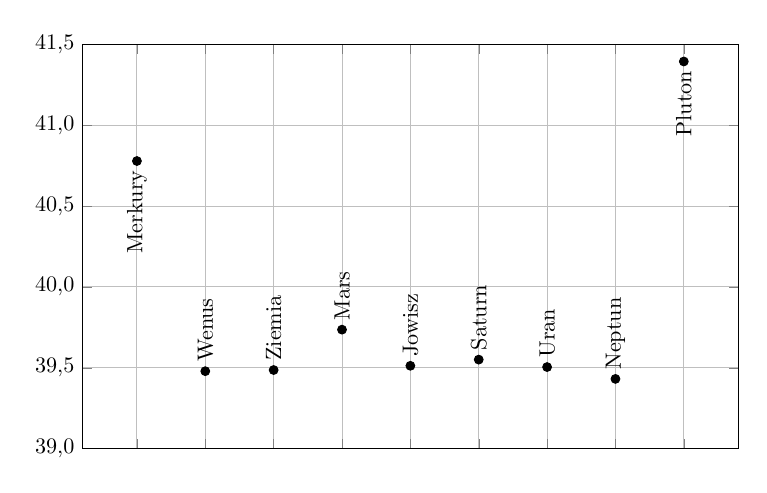
\begin{tikzpicture}[scale=.8]
    \begin{axis}[
        % title={Planetary Data},
        xlabel={},
        % xlabel={Ciała niebieskie},
        % ylabel={$\frac{GM_sT_o^2}{a^3}$},
        % ylabel style={rotate=-90, at={(0.02,0.7)}},
        xtick={1,2,3,4,5,6,7,8,9},
        xticklabels={},
        ytick={3.90, 3.95, 4.00, 4.05, 4.10, 4.15},
        yticklabels={39{,}0, 39{,}5, 40{,}0, 40{,}5, 41{,}0, 41{,}5},
        ymin=3.90, ymax=4.15,
        grid=both,
        width=12cm,
        height=8cm
    ]
    \addplot[
        only marks,
        mark=*,
        mark size=2pt
    ] coordinates {
    (1, 4.077850621616459)
    (2, 3.947906419282189)
    (3, 3.948621433096381)
    (4, 3.9735822373369696)
    (5, 3.95122428727248)
    (6, 3.955054303634854)
    (7, 3.9504572394466804)
    (8, 3.9431207878373344)
    (9, 4.139402324061695)
    };
    \pgfplotsextra{
        \foreach \x/\y/\label in {2/3.9479/Wenus, 3/3.9486/Ziemia, 4/3.9736/Mars, 5/3.9512/Jowisz, 6/3.9551/Saturn, 7/3.9505/Uran, 8/3.9431/Neptun} {
            \node[anchor=west, rotate=90] at (axis cs:\x, \y+0.001) {\label};
        }
        \foreach \x/\y/\label in {1/4.0779/Merkury, 9/4.1394/Pluton} {
            \node[anchor=east, rotate=90] at (axis cs:\x, \y-0.001) {\label};
        }
    }
    \end{axis}
\end{tikzpicture}}
 
Przyglądając się powyższemu diagramowi, widzimy, że przeprowadzone obliczenia rzeczywiście potwierdzają teorię Newtona. Większe odchylenia dla Merkurego
i~Plutona od stałej granicznej $4\pi^2$ wynikają z ich dużych mimośrodów.

Możemy teraz powrócić do wzoru (\ref{invariance1}). Dokonując prostego rachunku na wzorze (\ref{piękny}), możemy napisać wzór (\ref{invariance1}) w~ostatecznej formie jako\vspace*{2pt}
\begin{equation}\label{invariance3}
   \frac{GM_sT_o^2}{a^3} =
  \frac{4\pi^2}
  {1+\frac{m}{M_s}}.\vspace*{2pt}
\end{equation} 
Wzory (\ref{piękny}) i~(\ref{invariance3}) są równoważne i~oba reprezentują trzecie prawo Keplera. Ze wzorów (\ref{invariance1}) i~(\ref{invariance3}) wynika, że stała $\psi(1,0)$ jest równa $4\pi^2$. 
\end{dwieszpalty}

{\scriptsize
\hspace*{-5.5cm}\begin{tabular}{@{}l@{\qquad}l}
\includegraphics[width=0.45\textwidth]
{harm-poly-photo-1} 
\includegraphics[width=0.45\textwidth]{harm-poly-photo-2}&

\includegraphics[width=0.45\textwidth]{Harm-mus-photo2} \\[8pt]
Pomysły \add{Keplera} z~wielościanami&Układ planet i~harmonie w~muzyce
                \end{tabular}
                }\eject

Gwoli ścisłości historycznej należy powiedzieć, że nie ma pewności co do tego, jak Kepler rozumiał swoje trzecie prawo,
\marg{
Prowadzone są dyskusje, jak rozszyfrować oryginalne sformułowanie   trzeciego prawa Keplera. \\[1mm]
{\it Jest jednak całkowicie pewne i~dokładne, że stosunek czasów okresowych dowolnych dwóch planet jest dokładnie stosunkiem potęgi 3/2 średnich odległości, to jest samych kul; pod warunkiem jednak, że średnia arytmetyczna obu średnic orbity eliptycznej będzie nieco mniejsza niż dłuższa średnica.} ,,Harmonices Mundi''
}
gdyż w~,,Harmonices Mundi'' nie określa on w~jasny sposób, co rozumie przez ,,średnią odległość'', a~zgodność jego oryginalnego trzeciego prawa z~{jego} pomiarami orbitalnymi ruchu planet dotyczyła tylko orbit o~bardzo małych mimośrodach. Jak wspomnieliśmy, Merkury sprawiał mu kłopot, podobnie jak później wielu innym [Dembny,~2023]. Oryginalne sformułowanie Keplera nie mogło być sformułowaniem~(\ref{invariance3}), gdyż nie występuje w~nim mimośród, natomiast w~zasadzie  mogło być  sformułowaniem~(\ref{piękny}). %W~artykule nie wyklucza ono Merkurego.
W~artykule [Vijaya, 2019] można znaleźć wnikliwą rekonstrukcję rozumowania Keplera, prowadzącą do propozycji oryginalnej keplerowskiej ,,średniej odległości''.
\normalsize
  
Oczywiście Kepler nie wiedział jeszcze nic o~Uranie i~Plutonie. (Pluton został wykreślony z~listy planet przez
% wykluczony z~układu planet przez
Międzynarodową Unię Astronomiczną, IAU, 
bez zgodnego poparcia społeczności, nie tylko astronomów, w~2006 roku).\marg[-25]{
Średnia odległość planety od Słońca względem zmiennej $p$ wyraża się poprzez całkę
\[
r_p=\frac{1}{p}\int r(p)dp, 
\]
gdzie $r$ jest promieniem wodzącym planety po orbicie eliptycznej. Na~przykład średnie mierzone względem czasu ($t$), długości łuku ($s$) i~kąta obrotu ($\theta$) dla ruchu po okręgu z~centrum pola sił w~jego centrum są równe sobie (równe promieniowi okręgu), natomiast dla elipsy o~półosiach $a$, $b$ różnią się od siebie, \\
$r_t = a(1+e^2/2)$, $r_s=a$, $r_{\theta}=b$,
[Stein, 1977].
}

%%%%%%%%%
%https://www.astronomy.com/science/is-pluto-a-planet-%the-experts-break-it-down/
%%%%%%%%%

{\bf Krótkie podsumowanie metody analizy wymiarowej.} W~rozważanym powyżej zagadnieniu najpierw wyodrębniliśmy {\it istotne} dla jego rozwiązania wielkości fizyczne. Następnie {\it przyjęliśmy} długość, masę i~czas jako wielkości fundamentalne, a~stałą grawitacji jako wielkość pochodną, dającą się przedstawić jako iloczyn potęg wielkości fundamentalnych. Dalej {\it postulowaliśmy} istnienie pewnej relacji między istotnymi wielkościami, {\it niezmienniczej} ze względu na skalowanie. Korzystając z~niezmienniczości tej relacji, otrzymaliśmy, poprzez odpowiednie skalowanie, relację wiążącą ze sobą trzy bezwymiarowe wielkości.
Relacja ta zawierała w~sobie trzecie prawo Keplera.
{\it Matematyczne uzasadnienie} przeprowadzonych operacji jest zawarte w~najważniejszym twierdzeniu metody analizy wymiarowej, tzw. {\bf Twierdzeniu $\Pi$}, [Barenblatt, 2003], [Birkhoff, 1960], [Cantwell, 2002].

Powyższy przykład pokazuje zarówno siłę, jak i~pewne ograniczenia analizy wymiarowej.
O~sile tej metody świadczy to, że przy jej pomocy wyprowadziliśmy trzecie prawo Keplera, niewiele wiedząc o~fizyce zagadnienia. Metoda ta pozwala znaleźć prawidłową odpowiedź w~rozmaitych sytuacjach, gdy nie mamy wielu danych. Potrzebna jest natomiast świadomość pozwalająca założyć czy zgadnąć, od jakich wielkości ta odpowiedź może zależeć.
Zauważmy, że gdybyśmy w~definicji $\Pi_3$ użyli masy planety, a~nie masy Słońca, to obliczenia dla lewej strony wzoru (\ref{piękny}) byłyby rozstrzelone. Sama analiza wymiarowa nie podpowiada, który wybór, $M_s$ czy $m$, jest właściwy. Potrzebna zatem jest wiedza i~intuicja fizyczna. Ten fakt świadczy o~pewnym ograniczeniu analizy wymiarowej. 

We wstępie do monografii [Barenblatt, 2003] (patrz też uzupełniający materiał filmowy) przedstawiony jest przykład pokazujący, jak w~rękach takich uczonych jak Geoffrey I. Taylor i~John von Neumann analiza wymiarowa pozwoliła oszacować mechaniczny efekt eksplozji atomowej. Był rok 1940 i~była to bardzo cenna informacja dla celów wojennych. 
Ciekawe przykłady zastosowań analizy wymiarowej w~matematyce i~fizyce są przytoczone w~artykule [Wójcik, 2024].

\vspace*{\parskip}
\begin{dwieszpalty}
  \Magenta{\bf Ogólne uwagi o~analizie wymiarowej w~fizyce}
  
Poniżej przedstawiamy kilka ogólnych uwag dotyczących analizy wymiarowej w~fizyce, w~szerszym kontekście modelowania matematycznego.

W~fizyce nie ma uniwersalnych fundamentalnych wielkości, są one sprawą wygody i~konwencji, nawet w~danej teorii fizycznej. Przyjmowane w~mechanice newtonowskiej długość ($L$), masa ($M$) i~czas ($T$) jako wielkości fundamentalne to też tylko wybór. Sam Newton wolał wybrać pęd ($P$), siłę ($F$) i~prędkość~($V$).
Przy takim wyborze długość, masa i~czas są wielkościami pochodnymi, z~${L=PF^{-1}V}$, 
$M=PV^{-1}$ i $T=PF^{-1}$. Zwróćmy też uwagę, że
w~układzie~SI jednostki masy, długości i~czasu są zdefiniowane w~kategoriach konkretnych wielkości działania, prędkości i~częstości, które wtedy powinniśmy przyjąć jako wielkości podstawowe [Grozier, 2020].

Zakłada się, że w~fizyce wszystkie prawa powinny być niezależne od wyboru jednostek, czyli móc być wyrażone w~postaci bezwymiarowej. 
\marg{
Nie wchodzimy tu w~głębsze rozważania dotyczące tego {\it metafizycznego} założenia (jest ono dyskutowane np. w~[Birkhoff, 1960], [Grozier, 2020]). W~fizyce pozorna ,,oczywistość'' danego założenia nie może być dowodem na jego prawdziwość czy uniwersalność. Newtonowska niezależność czasu i~przestrzeni to przykład pozornie oczywistego założenia. Już Leibniz się z~tym założeniem nie zgadzał, ale trzeba było długo czekać, aby potwierdzić, że tego założenia nie można przyjąć jako uniwersalnej prawdy o~rzeczywistości fizycznej.
}
W~swoim magnum
opus James Clerk Maxwell napisał:
{\it Równania, do których dochodzimy, muszą być takie, aby osoba dowolnego narodu, zastępując różne symbole wartościami liczbowymi wielkości mierzonych w~jego własnych jednostkach narodowych, uzyskała prawdziwy wynik} [Maxwell, ,,Treatise'' (1873), art. 2]. Wcześniej, w~1822 roku, zwrócił też na ten wymóg uwagę Joseph Fourier  w~,,Théorie Analytique de la Chaleur''. Fourier jako pierwszy stwierdził, że istnieją pewne ,,jednostki podstawowe'', w~kategoriach których każda wielkość fizyczna ma pewne ,,wymiary''  możliwe do zapisania jako wykładniki.
Jeszcze wcześniej Galileusz i~Newton posługiwali się elementami analizy wymiarowej w~pewnych rozumowaniach [Birkhoff, 1960].

Niezależność praw fizyki od wyboru jednostek to inaczej ich niezmienniczość ze względu na grupę transformacji skalowania. Wiemy, że np. równania mechaniki Newtona są też niezmiennicze ze względu na grupę transformacji Galileusza. 
Grupy transformacji, 
względem których dane równanie jest niezmiennicze, nazywamy grupami symetrii tego równania [Cantwell, 2002], [Łukaszewicz, 2021].
Analiza wymiarowa jest tylko częścią teorii symetrii równań (zarówno algebraicznych, jak i~różniczkowych), wyrażających prawa fizyki w~ramach rozmaitych jej modeli (np.~mechaniki klasycznej, hydrodynamiki, mechaniki kwantowej). Symetrie są niezwykle ważne w~całej fizyce, są ściśle związane z~zasadą najmniejszego działania i~prawami zachowania.
\bigskip

{\small\parskip0pt\everypar={\hangindent20pt }
G. I. Barenblatt, {\it Scaling}, CUP, 2003. https://www.youtube.com/watch?v=wr-e9rGWx0c

G. Birkhoff, {\it Hydrodynamics. A~Study in Logic, Fact and Similitude}, Princeton University Press, 1960.

B. Cantwell, {\it Introduction to Symmetry Analysis}, CUP, 2002.

M. Dembny, I. Palusiński, G. Łukaszewicz, {\it Uran, Neptun i~Wulkan -- trzy planety, z~których jedna nigdy nie istniała}, cz. III, \ddlink{https://deltami.edu.pl/2023/11/uran-neptun-i-wulkan-trzy-planety-z-ktorych-jedna-nigdy-nie-istniala-cz-iii/}{11}{23}.

J. Grozier, {\it Should physical laws be unit-invariant?}, ,,Studies in the history and philosophy of science'' Part A, Vol. 80 (2020), str. 9--18. 

Gopi Krishna Vijaya, {\it Original form of Kepler's Third Law and its misapplication in Propositions XXXII-XXXVII in Newton's Principia (Book I)}, ,,Heliyon'' 5 (2019), 
\href{https://doi.org/10.1016/j.heliyon.2019.e01274}{DOI: 10.1016/j.heliyon.2019.e01274}.

G. Łukaszewicz, {\it Równania różniczkowe i~geometria, II}, \ddlink{https://deltami.edu.pl/2021/07/rownania-rozniczkowe-i-geometria-ii/}{7}{21}.

Sherman K. Stein, {\it ,,Mean Distance'' in Kepler's Third Law}, ,,Mathematics Magazine'', Vol. 50, no. 3, 160--162 (1977).

A. Wójcik, {\it Czy metr może być kwadratowy?}, \ddlink{https://deltami.edu.pl/2024/05/czy-metr-moze-byc-kwadratowy/}{5}{24}.

}
\end{dwieszpalty}

\input 08-lehman